\section{寄存器描述}
\regover{
{\hyperref[gpip-gpdac-config]{gpdac\_config}}&
\\
\hline
{\hyperref[gpip-gpdac-dma-config]{gpdac\_dma\_config}}&
\\
\hline
{\hyperref[gpip-gpdac-dma-wdata]{gpdac\_dma\_wdata}}&
\\
\hline
{\hyperref[gpip-gpdac-tx-fifo-status]{gpdac\_tx\_fifo\_status}}&
\\
\hline
}


\subsection{gpdac\_config}
\label{gpip-gpdac-config}
地址:0x20002040
 \begin{figure}[H]
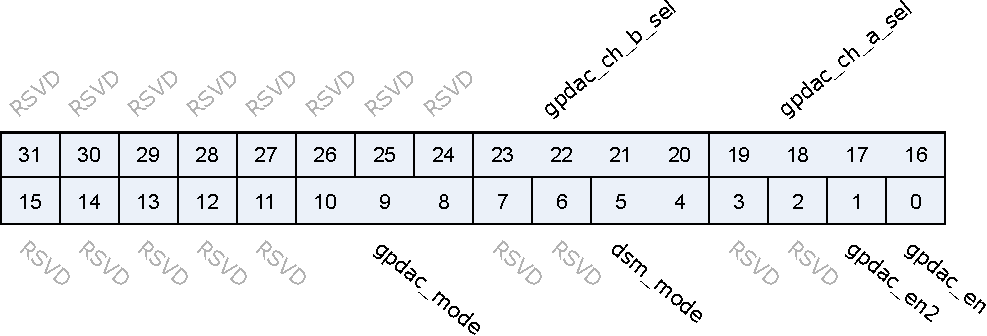
\includegraphics{gpip_gpdac_config.pdf}
\end{figure}

\regdes{31:24&rsvd&rsvd&8'h0d&\\\hline
23:20&gpdac\_ch\_b\_sel&r/w&0&Channel B Source Select \par 0: Reg \par 1: DMA \par 2: DMA + Filter \par 3: Sin Gen \par 4: A (The same as channel A) \par 5: ~A (Inverse of channel A)
\\\hline
19:16&gpdac\_ch\_a\_sel&r/w&0&Channel A Source Select \par 0: Reg \par 1: DMA \par 2: DMA + Filter \par 3: Sin Gen
\\\hline
15:11&RSVD& & & \\\hline
10:8&gpdac\_mode&r/w&0&0:32k, 1:16k, 3:8k,  4:512k(for DMA only)\\\hline
7:1&RSVD& & & \\\hline
0&gpdac\_en&r/w&0&GPDAC enable\\\hline

}
\subsection{gpdac\_dma\_config}
\label{gpip-gpdac-dma-config}
地址:0x20002044
 \begin{figure}[H]
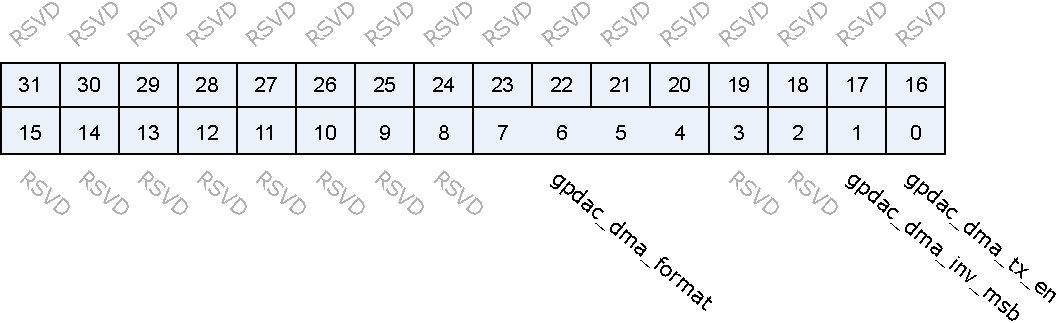
\includegraphics{gpip_gpdac_dma_config.pdf}
\end{figure}

\regdes{31:8&RSVD& & & \\\hline
7:4&gpdac\_dma\_format&r/w&0&DMA TX format (Data 10-bit) \par 0: ([9:0]) {A0}, {A1}, {A2}… \par 1: ([25:16][9:0]) {B0,A0}, {B1,A1}, {B2,A2}… \par 2: ([25:16][9:0]) {A1,A0}, {A3,A2}, {A5,A4}… \par 4: ([15:6]) {A0}, {A1}, {A2}… \par 5: ([31:22][15:6]) {B0,A0}, {B1,A1}, {B2,A2}… \par 6: ([31:22][15:6]) {A1,A0}, {A3,A2}, {A5,A4}… \par 8: ([31:24][23:16][15:8][7:0]) {A3,A2,A1,A0}, {A7,A6,A5,A4}… \par 9: ([31:24][23:16][15:8][7:0]) {B1,B0,A1,A0}, {B3,B2,A3,A2}… \par 10: ([31:24][23:16][15:8][7:0]) {B1,A1,B0,A0}, {B3,A3,B2,A2}… \par 11: ([15:8][7:0]) {B0,A0}, {B1,A1}, {B2,A2}…
\\\hline
3:2&RSVD& & & \\\hline
1&gpdac\_dma\_inv\_msb&r/w&0&GPDAC DMA Data Inverse MSB\\\hline
0&gpdac\_dma\_tx\_en&r/w&0&GPDAC DMA TX enable\\\hline

}
\subsection{gpdac\_dma\_wdata}
\label{gpip-gpdac-dma-wdata}
地址:0x20002048
 \begin{figure}[H]
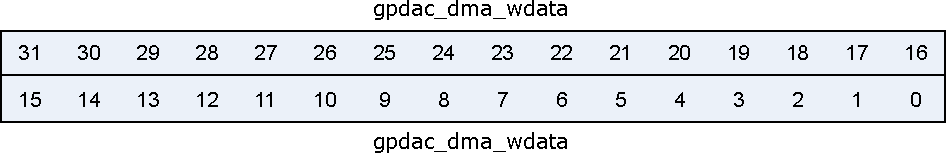
\includegraphics{gpip_gpdac_dma_wdata.pdf}
\end{figure}

\regdes{31:0&gpdac\_dma\_wdata&w&x&GPDAC DMA TX data\\\hline

}
\subsection{gpdac\_tx\_fifo\_status}
\label{gpip-gpdac-tx-fifo-status}
地址:0x2000204c
 \begin{figure}[H]
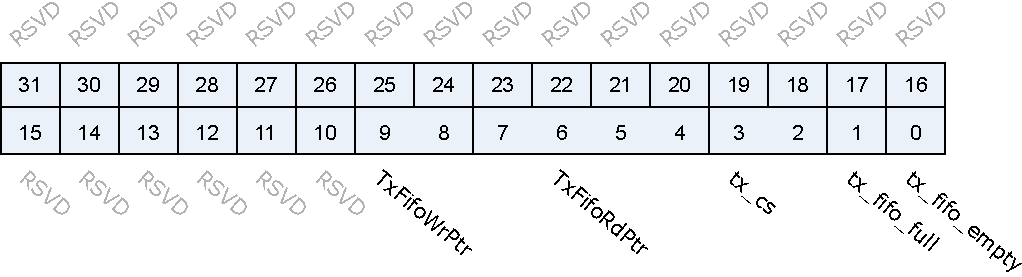
\includegraphics{gpip_gpdac_tx_fifo_status.pdf}
\end{figure}

\regdes{31:10&RSVD& & & \\\hline
9:8&TxFifoWrPtr&r&0&\\\hline
7:4&TxFifoRdPtr&r&4'd8&\\\hline
3:2&tx\_cs&r&0&\\\hline
1&tx\_fifo\_full&r&0&\\\hline
0&tx\_fifo\_empty&r&0&\\\hline

}
